The \gls{lhc}~\cite{LHC} is a two ring superconducting hadron accelerator and
collider located at the \gls{cern}.

The performance of a collider is evaluated in terms of its available
\emph{center of mass energy}, $\sqrt{s}$ and the \emph{instantaneous luminosity}
$\lumi$. The former defines the accessible energies for particle production. The
latter is defined as the interaction rate per unit cross section of the
colliding beams (collisions / (cm$^2$ s)).

The LHC is designed to operate at $\sqrt{s} = 14$~TeV in the center of mass
although it started off at 7~TeV in 2010 and 2011, 8~TeV in 2012 and 13~TeV in
2015 after the long shutdown in 2013 and 2014.

There are six experiments at LHC: ATLAS~\cite{ATLASPaper},
CMS~\cite{1748-0221-3-08-S08004}, ALICE~\cite{ALICE}, LHCb~\cite{LHCb},
LHCf~\cite{LHCf} and TOTEM~\cite{TOTEM}\@. ATLAS and CMS are designed to work
with the maximum luminosity that LHC can provide $\sim 10^{34}$~cm$^{-2}$
s$^{-1}$. This requirement, due to the low efficiency production, excludes the
use of anti-proton beams and therefore the LHC is designed to be a \gls{pp} and
heavy ions collider. The protons are organized in bunches, accelerated by LINAC2
to an energy of 50~MeV and subsequently injected in the \gls{psb}. Here they are
further accelerated to an energy of 1.4~GeV and fed to the \gls{ps} where they
reach the energy of 25~GeV to be then passed to the \gls{sps} which accelerate
them to an energy of 450~GeV. They are finally injected in the LHC in opposite
directions where they reach the nominal energy. There are four interaction
points where the four main experiments (ATLAS, CMS, ALICE, LHCb) are located, at
these locations, every 25~ns, the bunches cross and interact with each other
(\emph{bunch crossing}). A schematic view of the injection chain is depicted in
Figure~\ref{fig:lhc_inj_chain}.

The instantaneous luminosity depends on the beam parameters and is given by:
\begin{equation}
  \label{eq:70}
  \lumi = \frac{N^2_b n_b f_{rev} \gamma}{4 \pi \epsilon_n \beta^*} F
\end{equation}
where $N_b$ is the number of particles per bunch, $n_b$ is the number of bunches
per beam, $f_{rev}$ is the revolution frequency, $\gamma$ is the relativistic
gamma factor, $\epsilon_n$ the normalized transverse beam emittance, the beta
function is a measure of the transverse beam size and $\beta^*$ is the value of
the beta function at the interaction point and $F$ is the geometric reduction
factor due to the crossing angle of the beams at the \gls{ip}~\cite{LHC}. The
integrated luminosity is given by:
\begin{equation}
  \label{eq:71}
  L = \int \lumi \ud t
\end{equation}
and the integral is carried over data taking periods of the detector. The
integrated luminosity can be related to the total number of events of a certain
process by:
\begin{equation}
  \label{eq:72}
  N_{events} = L \sigma_{events}
\end{equation}
where $N_{events}$ is the total number of events, $L$ is the integrated
luminosity and $\sigma_{events}$ is the cross section for the process in units
of barn (1~b = 10$^{-28}$~m$^2$). In 2015 ATLAS recorded an integrated
luminosity of 3.2~\ifb.

\begin{figure}[!h]
  \centering
    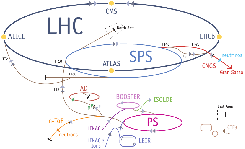
\includegraphics[width=.8\linewidth]{lhc_inj_chain}
    \caption{The LHC injection chain~\cite{LHCFAQ}.}
    \label{fig:lhc_inj_chain}
\end{figure}
%%% Local Variables:
%%% mode: latex
%%% TeX-master: "../search_for_DM_LED_with_ATLAS"
%%% End:
